\documentclass[a4paper,11pt,landscape,twocolumn]{article}

\usepackage{préambule}
\usepackage{clipboard}

\makeatletter
\renewcommand{\maketitle}{%
{\scriptsize colle dans ton cahier d'exercices}
	\begin{center}
		\LARGE
		\uline{\@title}
		\vspace{0.5em}
	\end{center}
}
\makeatother

\title{Activité : Égalité de fraction}
\date{}
\author{}

\begin{document}

\Copy{Activite}{
\maketitle

Pour chaque grille, place la/les fractions qui lui correspondent dans la case en dessous.

\vspace{0.5em}

\begin{center}
	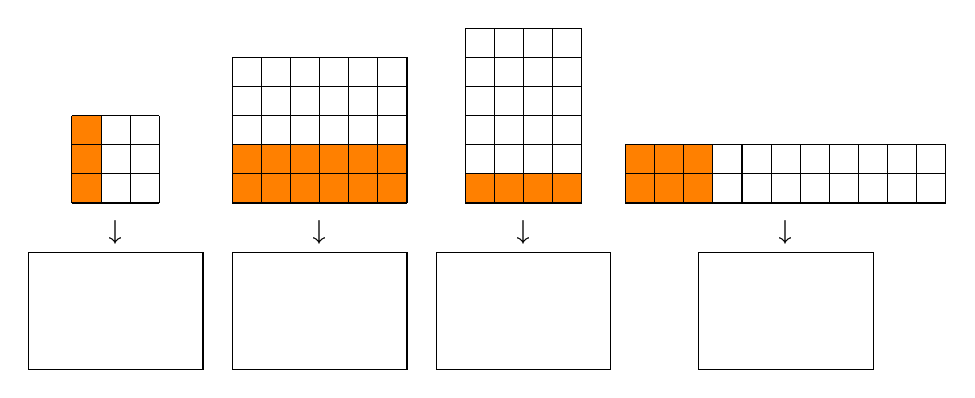
\begin{tikzpicture}[scale=0.37]
		\def\A{0};
		\def\B{7};
		\def\C{14};
		\def\D{23};

		\fill[orange] (\A+1.5,0) rectangle ++(1,3);
		\draw[xshift=0.5cm] (\A+1,0) grid ++(3,3);
		\node at (\A+3,-1) {↓};
		\draw (\A,-1.7) rectangle ++(6,-4);

		\fill[orange] (\B,0) rectangle ++(6,2);
		\draw (\B,0) grid ++(6,5);
		\node at (\B+3,-1) {↓};
		\draw (\B,-1.7) rectangle ++(6,-4);

		\fill[orange] (\C+1,0) rectangle ++(4,1);
		\draw (\C+1,0) grid ++(4,6);
		\node at (\C+3,-1) {↓};
		\draw (\C,-1.7) rectangle ++(6,-4);

		\fill[orange] (\D-2.5,0) rectangle ++(3,2);
		\draw[xshift=0.5cm] (\D-3,0) grid ++(11,2);
		\node at (\D+3,-1) {↓};
		\draw (\D,-1.7) rectangle ++(6,-4);
	\end{tikzpicture}
\end{center}

\vspace{1.5em}

\renewcommand{\arraystretch}{3}
\begin{center}
	\begin{tabular}{llll}
		$\cfrac{1}{3}$ \hspace{3em} & $\cfrac{12}{30}$ \hspace{3em} & $\cfrac{4}{24}$ \hspace{3em} & $\cfrac{12}{44}$ \\
		$\cfrac{6}{22}$             & $\cfrac{3}{9}$                & $\cfrac{2}{12}$              & $\cfrac{6}{18}$  \\
		$\cfrac{4}{10}$             & $\cfrac{3}{11}$               & $\cfrac{1}{6}$               & $\cfrac{2}{5}$   \\
		                            & $\cfrac{10}{60}$              & $\cfrac{6}{15}$              &                  \\
	\end{tabular}
\end{center}
}

\newpage

\Paste{Activite}


\end{document}